\documentclass[a4paper,12pt]{article}
\usepackage[12pt]{extsizes}




\usepackage{cmap}					% поиск в PDF
\usepackage{mathtext} 				% русские буквы в формулах
\usepackage[T2A]{fontenc}			% кодировка
\usepackage[utf8]{inputenc}			% кодировка исходного текста
\usepackage[english,russian]{babel}	% локализация и переносы
\usepackage{ulem}                   % зачеркнутый текст
\usepackage{amssymb}			% пакет математики
\usepackage{float}
\usepackage{amsmath}
\usepackage{graphicx}
\DeclareGraphicsExtensions{.png}

%%% Страница
%\usepackage{extsizes} % Возможность сделать 14-й шрифт
\usepackage[left=1cm,right=1cm,top=1cm,bottom=1cm]{geometry} % Простой способ задавать поля
\pagestyle{empty}

\begin{document}


\begin{center}
ФЕДЕРАЛЬНОЕ ГОСУДАРСТВЕННОЕ ОБРАЗОВАТЕЛЬНОЕ БЮДЖЕТНОЕ УЧРЕЖДЕНИЕ ВЫСШЕГО ОБРАЗОВАНИЯ

    \textbf{«ФИНАНСОВЫЙ УНИВЕРСИТЕТ ПРИ ПРАВИТЕЛЬСТВЕ РОССИЙСКОЙ ФЕДЕРАЦИИ»}

Факультет информационных технологий и анализа больших данных

Департамент анализа данных и машинного обучения

\textit{
	\textbf{Дисциплина: «Теория вероятностей и математическая статистика»}}

\textit{Направление подготовки: 01.03.02 «Прикладная математика и информатика»}

\textit{Профиль: «Анализ данных и принятие решений в экономике и финансах»}

\textit{Форма обучения очная, учебный 2020/2021 год, 4 семестр}

\textbf{Билет 113}

\end{center}

\begin{enumerate}


\item


Сформулируйте определение случайной выборки из конечной генеральной совокупности. Какие
виды выборок вам известны? Перечислите (с указанием формул) основные характеристики выборочной и генеральной совокупностей


\item

Случайные величины $X$ и $Y$ независимы и имеют равномерное
распределение на отрезках $[0;10]$ и $[0;3]$ соответственно. Для случайной величины $Z=\frac{Y}{X}$ найдите: 
1) функцию распределения $F_Z(x)$;
2) плотность распределения $f_Z(x)$ и постройте график плотности;
3) вероятность $\P(0,\!057\leqslant Z\leqslant 0,\!556)$.


\item


(10) Известно, что доля возвратов по кредитам в банке имеет распределение $F(x) = x ^{\beta}, 0 \leqslant x \leqslant 1$.
Наблюдения показали, что в среднем она составляет $75,0\%$. Методом моментов оцените параметр $\beta$ и
вероятность того, что она опуститься ниже $20\%$


\item

    
    Создайте эмперические совокупности  $\mathtt{\text{exp}}$ и $\mathtt{\text{log}}$ вида $\mathtt{\text{exp}}(1),\mathtt{\text{exp}}(2), ..., \mathtt{\text{exp}}(77) $ и $\mathtt{\text{log}}(1),\mathtt{\text{log}}(2), ..., \mathtt{\text{log}}(77). $

    Найдите эмпирическое среднее и эмпирическое стандартное отклонение совокупности $\mathtt{\text{exp}}$, её четвёртый эмпирический центральный момент и эмпирический эксцесс.

    Кроме того, найдите эмпирический коэффициент корреляции признаков $\mathtt{\text{exp}}$ и $\mathtt{\text{log}}$ на совокупности натуральных чисел от $1$ до $77$.
    

\item

    
    	Распределение результатов экзамена в некоторой стране с $14$-балльной системой оценивания задано следующим образом:
    	$\left\{ 1 : 3, \  2 : 7, \  3 : 5, \  4 : 2, \  5 : 11, \  6 : 9, \  7 : 2, \  8 : 19, \  9 : 23, \  10 : 26, \  11 : 15, \  12 : 9, \  13 : 20, \  14 : 41\right\}$

	Работы будут перепроверять $16$ преподавателей, которые разделили все имеющиеся работы между собой случайным образом. Пусть $\overline{X}$ - средний балл (по перепроверки) работ, попавших к одному преподавателю.

	Требуется найти матожидание и стандартное отклонение среднего балла работ, попавших к одному преподавателю, до перепроверки.
    

\item


(10) Пусть $X _{1}$, $X _{2}$, $X _{3}$, $X _{4}$ выборка из $N(\theta, \sigma ^{2})$. Рассмотрим две оценки параметра $\theta$:
\[\hat \theta _{1} = \frac{X _{1} + X _{2} + X _{3} + 7X _{4}}{10}, \hat \theta _{1} = \frac{3X _{1} + 5X _{2} + X _{3} + X _{4}}{10}\]
a) Покажите, что обе оценки несмещенные.
б) Какая из оценок оптимальная?


\end{enumerate}

\begin{figure}[H]
	Подготовил
	\hfill
	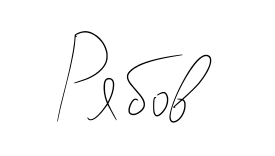
\includegraphics[width=2cm]{Prepared}
	П.Е. Рябов
\end{figure}


\begin{figure}[H]
	Утверждаю:\\
	Первый заместитель\\
	руководителя департамента\\
	Дата 01.06.2021
	\hfill
	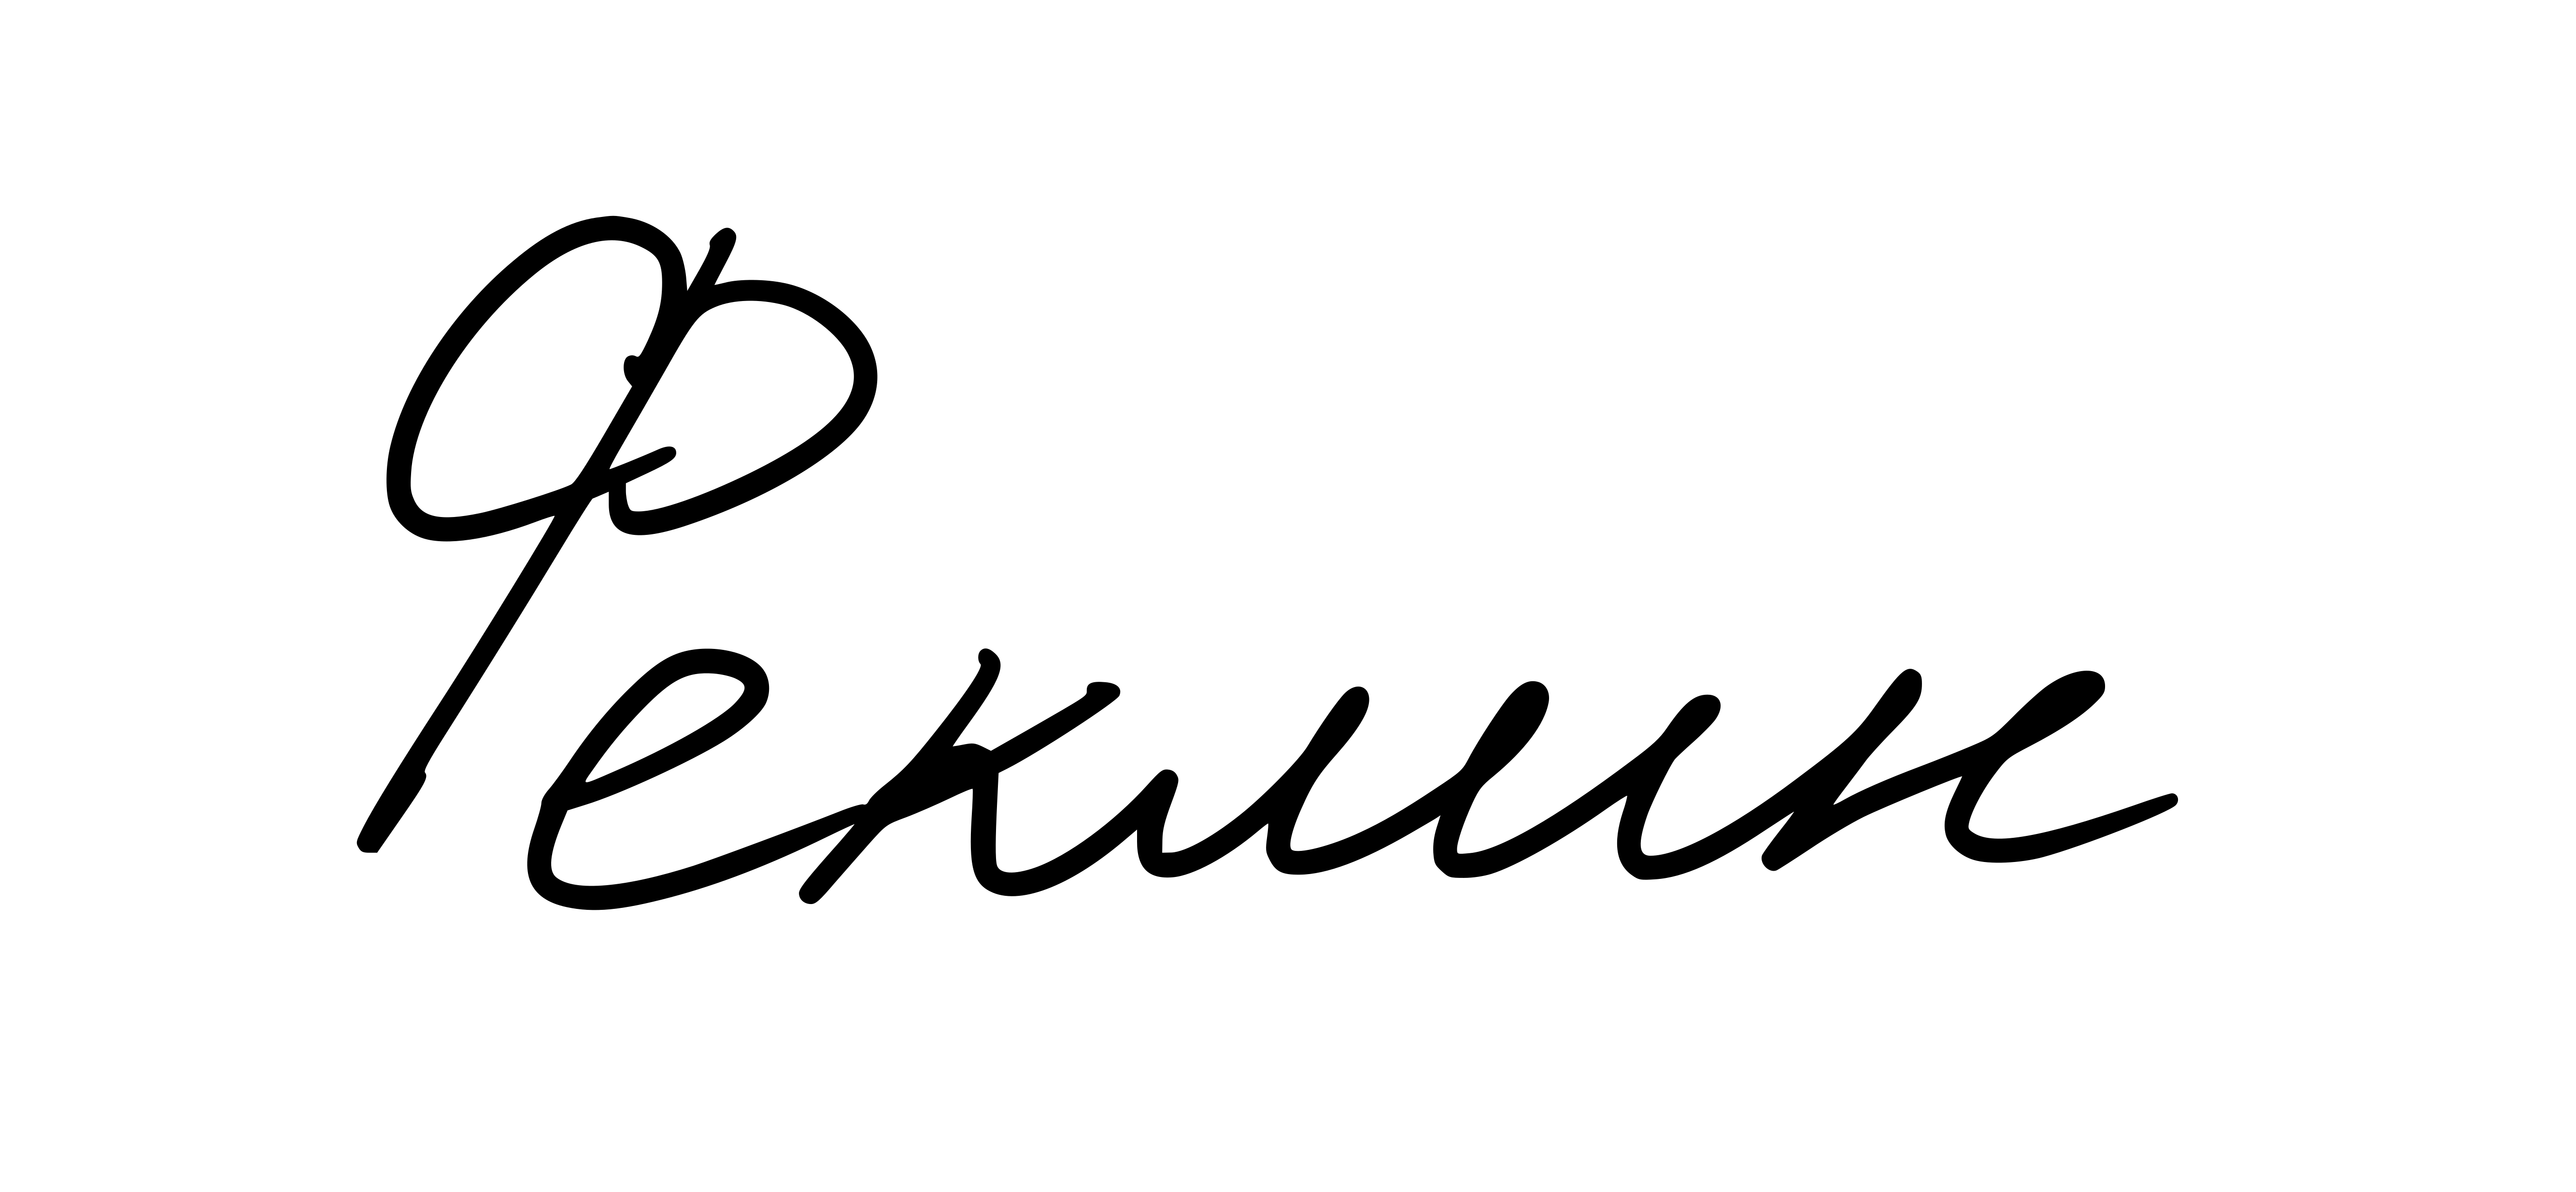
\includegraphics[width=2cm]{Approved}
	Феклин В.Г.
\end{figure}

\end{document}

